\subsubsection{Задача № 1367.}

Линейное подпространство $L$ задано уравнениями :
$$
\begin{cases}
    2x_1  + x_2 + 3x_3 -x_4 = 0\\
    3x_1 + 2x_2 -2x_4 = 0\\
    3x_1 +x_2 + 9x_3-x_4=0
\end{cases}$$
Найти уравнение задающее $L^\perp$ и само $L^\perp$

\textbf{Решение:}

Давайте найдем $L$. Для этого решим соответствующую СЛОУ. 

Получим $L = \span (\begin{pmatrix}
    -6 \\
    9 \\
    1\\0
    
\end{pmatrix}, \begin{pmatrix}
    0 \\
    1\\
    0\\
    1\\
\end{pmatrix})$.

Теперь, чтобы задать $L^\perp$ я получаю такую СЛОУ(так как скалярное с $\forall x \in L^\perp$ должно быть нулем):
$$\begin{pmatrix}[cccc|c]
    -6 & 9 & 1 & 0 & 0\\
    0 & 1 & 0 & 1 & 0
\end{pmatrix}$$
Решим и получим: $L^\perp = \span (\begin{pmatrix}
    1 \\ 0
    \\ 6\\0
\end{pmatrix},\begin{pmatrix}
    -3 \\
    -2 \\
    0\\
    2
\end{pmatrix})$

Можно проверить, что наши вектора делают то, что надо, но это и так видно.
\subsubsection{Задача № 1371}

Найти ортогональную проекцию $y$ и ортогональную составляющую $z$ вектора $x$ на линейное подпространство $L$.

$x = \begin{pmatrix}
    5 \\
    2\\-2\\2
\end{pmatrix}, L$ натянуто на векторы $a_1 = \begin{pmatrix}
    2 \\
    1\\
    1\\-1
\end{pmatrix}, a_2 = \begin{pmatrix}
    1\\
    1\\
    3\\
    0
\end{pmatrix}, a_3 = \begin{pmatrix}
    1 \\2\\8\\1
\end{pmatrix}$

\textbf{Решение:}

Давайте выделим базис сначала. Ранг системы векторов равен 2, поэтому возьму за базис $a_1,a_2$. Повторяя, процесс описанный в практике, получаю СЛОУ:
$$
\begin{cases}
    (x,a_1) = c_1(a_1,a_1) + c_2(a_2,a_1)\\
    (x,a_2)  = c_1(a_1,a_3) + c_2(a_3,a_3)
\end{cases}
$$
Решая это простое СЛНУ найдем решение и получим ответ.

\subsubsection{Задача № 1374(а)}

Найти расстояние от точки, заданной вектором $x$, до линейного многообразия, заданнного системой векторов.

$$\begin{cases}
    x = \begin{pmatrix}
        4\\
        2\\
        -5\\
        1
    \end{pmatrix}\\
    2x_1 - 2x_2 + x_3 + 2x_4 = 9\\
    2x_1 - 4x_2 + 2x_3 + 3x_4 =12
\end{cases}$$

\textbf{Решение:}

Из теории $dist(x,P) = ||z||$, где $y+z =x -x_0$. Давайте найдем линейное многообразие:

$P = \begin{pmatrix}
    3 \\
    -\cfrac{3}{2}\\
    0\\
    0
\end{pmatrix} + t_1 \begin{pmatrix}
    0 \\
    \cfrac{1}{2}\\
    1\\
    0
\end{pmatrix} + t_2 \begin{pmatrix}
    -\cfrac{1}{2}\\
    \cfrac{1}{2}\\
    0\\
    1
\end{pmatrix}$

А дальше мы уже проделывали аналогичные вещи в прошлой задаче, так что я пропущу это.

\subsubsection{Задача № 1377}

\begin{center}
   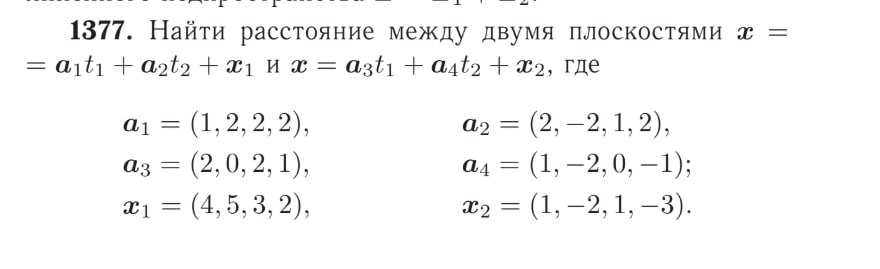
\includegraphics[width = 16cm]{assets/homework-5-task-1377.jpg}
\end{center}

Это делается крайне легко,  нужно лишь воспользоваться следствием, что 

$dist(P_1, P_2) = ||z||$, где $z$ ортогональная составляющая $x_1-x_2$ относительно $L= L_1 + L_2$.



